\documentclass{article}

\newcommand{\NomeDocumento}{Sistemi Concorrenti e Distribuiti}
\newcommand{\Versione}{1.0}

\usepackage{fancyhdr}
\usepackage{lastpage}
\usepackage{color}
\usepackage{graphicx}
\usepackage{midpage}
\usepackage{booktabs}
\usepackage{float}
\usepackage[italian]{babel}
\usepackage{hyperref}
\usepackage{lettrine}
\hypersetup{
  colorlinks,
  citecolor=black,
  filecolor=black,
  linkcolor=black,
  urlcolor=black
}

\pagestyle{fancy}

\lfoot{\bfseries \NomeDocumento}
\cfoot{}
\rfoot{\thepage/\pageref{LastPage}}
\renewcommand{\footrulewidth}{0.4pt}

\begin{document}

\begin{titlepage} % era midpage

\begin{center}

\begin{figure}[H]
\begin{center} % \centering

\includegraphics[ width=110px]{./img/Logo_Padova.png}
\label{Logo}
\end{center} % aggiunta
\end{figure}

\begin{center}
 \vspace{1em}

 {\Large \textsc{Universit\`{a} degli Studi di Padova}}\\

\vspace{1em}

 {\Large \textsc{Corso di Laurea Magistrale in Informatica}}\\
 
 \vspace{5em}
 
 {\Large Sistemi Concorrenti e Distribuiti}\\

 \vspace{5em}

 {\LARGE \textbf{Traffico citt\`{a}}}\\

 \clearpage{\pagestyle{empty}\cleardoublepage} % puoi toglierlo, credo

\end{center}

\end{center}

\end{titlepage} % era midpage
\newpage
\null 
\newpage

\newpage
\begin{itemize}
\color{black}\item {Versione 1}
\color{green}\item {Versione 2}
\end{itemize}
\color{black}\emph{Modifiche:}
\begin{itemize}
\item {-}
\end{itemize}
\color{black}\emph{Aggiunte:}
\begin{itemize}
\item {Stesura documento}
\end{itemize}
\newpage

\tableofcontents 
\listoftables
\listoffigures
\newpage

\pagestyle{fancy}

\lhead{
	\color{black}
	\bfseries \textsf{\normalsize Introduzione\\} 
}
\chead{}
\rhead{
	\color{black}
	\bfseries \textsf{\normalsize v.\Versione\\} 
}
\section{Introduzione}
\lettrine[lines=1]{Q}{}uesto documento ha lo scopo di presentare il lavoro svolto per il corso di Sistemi Concorrenti e Distribuiti per il corso di Laurea Magistrale in Informatica. 
\par Verr\`{a} presentata inizialmente una breve descrizione del problema, seguita poi dall\textquoteright{}analisi di tale problema e dalla presentazione di una delle possibili implementazioni.
\subsection{Problema}
\lettrine[lines=1]{I}{}l problema consiste nello studio e nell\textquoteright{}implementazione di sistema rappresentante una citt\`{a} con i suoi residenti. La citt\`{a} deve gestire in maniera corretta tutti gli aspetti di concorrenza e di distribuzione. Requisiti obbligatori sono dunque la distribuzione e la scalabilit\`{a}. 

\newpage

\pagestyle{fancy}

\lhead{
	\color{black}
	\bfseries \textsf{\normalsize Esecuzione\\} 
}
\chead{}
\rhead{
	\color{black}
	\bfseries \textsf{\normalsize v.\Versione\\} 
}

\section{Esecuzione}
\lettrine[lines=1]{P}{}rima di illustrare per\`{o} lo studio fatto, verr\`{a} illustrato brevemente il software necessario per la corretta esecuzione dell\textquoteright{}applicazione.
\subsection{SBT}
\lettrine[lines=1]{S}{}BT \`{e} un build tool open source usato per progetti Scala e Java. Al momento, nonostate varie critiche, \`{e} il build tool pi\`{u} utilizzato per i progetti realizzati in Scala.
Per poter eseguire il progetto, sono stati offerti due diversi metodi. 

\par Il primo consente di eseguire tutto senza fornire alcun parametro. Baster\`{a} semplicemente avviare l\textquoteright{}esecuzione tramite il comando \textit{sbt run} come nella figura sotto riportata. In questo modo sar\`{a} l\textquoteright{}applicazione verr\`{a} eseguita con una sola JVM.

\begin{figure}[H]
\begin{center}
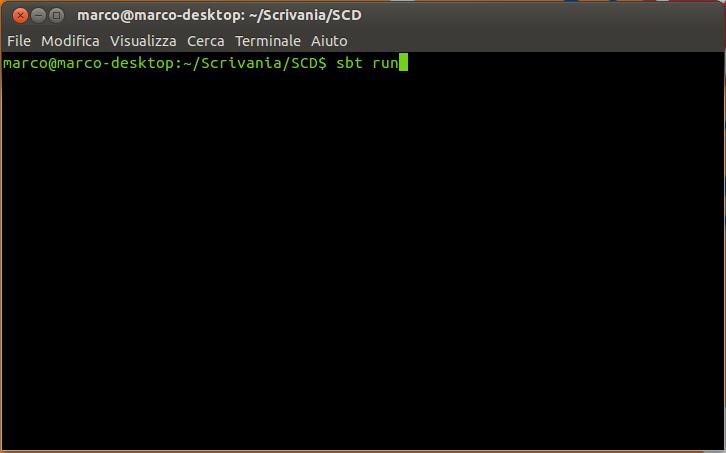
\includegraphics[ width=350px]{./img/SBT1.png}
\caption{Unica JVM}
\label{fig:Unica JVM}
\end{center}
\end{figure}

\par Il secondo consente invece di specificare l\textquoteright{}identificativo e la porta desiderata per ogni zona della citt\`{a}, la quale verr\`{a} quindi eseguita in una propria JVM differente. Questa modalit\`{a} \`{e} molto utile in quanto consentir\`{a} di \lq{}rimuovere\rq{} {} e \lq{}aggiungere\rq{} {} zone a piacimento, ma questo verr\`{a} spiegato meglio in seguito.

\begin{figure}[H]
\begin{center}
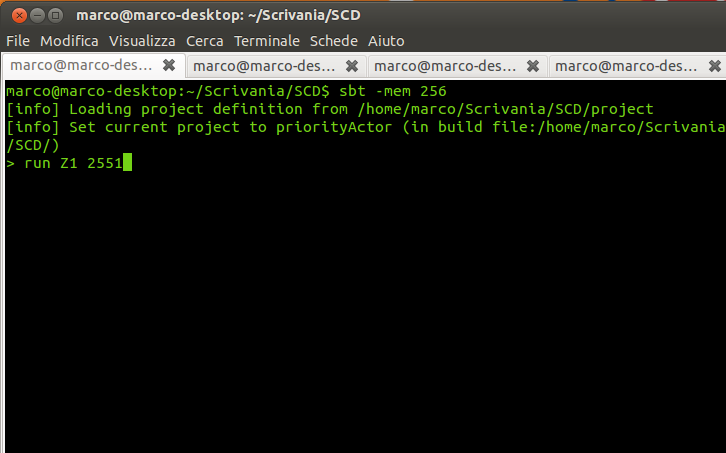
\includegraphics[ width=350px]{./img/SBT2.png}
\caption{Multiple JVM}
\label{fig:Multiple JVM}
\end{center} 
\end{figure}

\subsection{Scala ed Akka}
\lettrine[lines=1]{I}{}l linguaggio scelto per realizzare il progetto \`{e} Scala. Per l\textquoteright{}installazione del toolkit Akka baster\`{a} semplicemente specificare nel file di configurazione (\textit{build.sbt}) del progetto le \lq{}dipendenze\rq{} {}. In questo modo, alla prima esecuzione, SBT scaricher\`{a} tutto il necessario per la corretta esecuzione. 

\begin{figure}[H]
\begin{center}
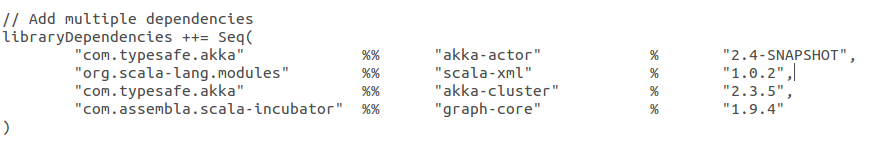
\includegraphics[ width=350px]{./img/build.png}
\caption{Build.sbt}
\label{fig:Build.sbt}
\end{center} 
\end{figure}

\newpage

\pagestyle{fancy}

\lhead{
	\color{black}
	\bfseries \textsf{\normalsize Studio del problema\\} 
}
\chead{}
\rhead{
	\color{black}
	\bfseries \textsf{\normalsize v.\Versione\\} 
}

\section{Studio del problema}
\subsection{Entit\`{a}}
\lettrine[lines=1]{I}{}l primo obbiettivo del progetto era decidere cosa bisognava distribuire e cosa no. Per poter raggiungerlo correttamente, \`{e} stata creata una gerarchia delle entit\`{a} che formano una citt\`{a}. 
\begin{itemize}
\item {Zone}
\item {Incroci}
\item {Strade/Marciapiedi}
\item {Fermate}
\item {Mezzi}
\item {Persone}
\end{itemize}
Si \`{e} dunque studiato quale delle entit\`{a} sopra elencate potesse essere distribuita.
\begin{itemize}
\item {Zone:} possono gestire molte cose internamente e comunicare solo per le cose essenziali
\item {Incroci, fermate, strade, marciapiedi, mezzi e persone:} richiedono molta comunicazione rispetto alle zone in quanto devono eseguire un insieme limitato di compiti
\end{itemize}
Distribuire le zone \`{e} sembrata dunque la scelta migliore.

Entrando nel dettaglio, sono poi state definite le varie entit\`{a}. Dato che il lavoro \`{e} stato svolto da una singola persona, sono state fatte delle scelte atte a non aumentare troppo la difficolt\`{a} del progetto. 
In primo luogo, la citt\`{a} \`{e} stata pensata come una griglia. Ogni cella di tale griglia contiene le varie strade, i vari marciapiedi ed eventualmente un incrocio. Tale citt\`{a} non verr\`{a} generata in maniera casuale, ma verr\`{a} creata all\textquoteright{}inizio dall\textquoteright{}utente. 
\begin{figure}[H]
\begin{center}
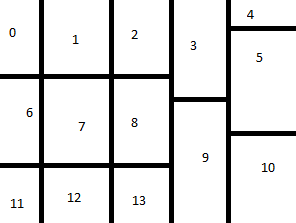
\includegraphics{./img/Citta.png}
\caption{Citt\`{a}}
\label{fig:Citt\`{a}}
\end{center}
\end{figure}
\begin{figure}[H]
\begin{center}
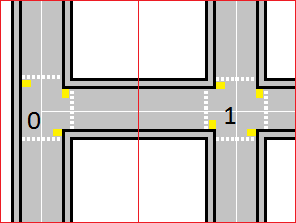
\includegraphics{./img/Zone.png}
\caption{Zone}
\label{fig:Zone}
\end{center}
\end{figure}
Come si vede dall\textquoteright{}immagine qui sopra, si \`{e} deciso di permettere ai pedoni di attraversare la strada solamente agli incroci. Per fare ci\`{o} ovviamente sar\`{a} necessaria una corretta gestione dei semafori, i quali funzioneranno nel seguente modo:
\begin{itemize}
\item {1:} Semafori rossi per i pedoni; Semafori verdi per alcune strade.
\item {2:} Semafori verdi per i pedoni; Semafori rossi per tutte le strade.
\item {3:} Semafori rossi per i pedoni; Semafori verdi per le altre strade strade.
\item {4:} Semafori verdi per i pedoni; Semafori rossi per tutte le strade.
\item {1:} Semafori rossi per i pedoni; Semafori verdi per alcune strade.
\item {2:} E cos\`{i} via...
\end{itemize}
Un\textquoteright{}altra limitazione aggiunta consiste nel mettere dei versi alle strade e ai marciapiedi. Le macchine ed i pedoni potranno procedere solamente nelle direzioni indicate nella figura sottostante.
\begin{figure}[H]
\begin{center}
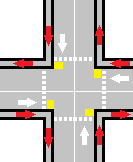
\includegraphics{./img/Direzioni.png}
\caption{Direzioni}
\label{fig:Direzioni}
\end{center}
\end{figure}
Si \`{e} deciso di creare all\textquoteright{}inizio anche i percorsi che dovranno seguire mezzi e pedoni. Le posizioni dei mezzi e dei pedoni verranno mostrate all\textquoteright{}arrivo negli incroci, all\textquoteright{}arrivo in una zona e all\textquoteright{}inizio di una strada/marciapiede.

\subsection{Stati}
Sono stati ora analizzati gli stati assunti dalle varie entit\`{a}.
\begin{itemize}
\item {Zona:}
\begin{itemize}
\item {1.} Creazione
\item {2.} Ricezione mezzi
\item {3.} Ricezione pedoni
\item {4.} Attesa
\item {5.} Instradamento mezzi
\item {6.} Instradamento pedoni
\end{itemize}
\item {Incrocio:}
\begin{itemize}
\item {7.} Gestione incrocio
\item {8.} Ricezione mezzi
\item {9.} Ricezione pedoni
\item {10.} Invio mezzi
\item {11.} Invio pedoni
\end{itemize}
\item {Corsia:}
\begin{itemize}
\item {12.} Invio mezzo
\item {13.} Ricezione mezzo
\item {14.} Attesa
\end{itemize}
\item {Marciapiede:}
\begin{itemize}
\item {15.} Invio pedone
\item {16.} Ricezione pedone
\item {17.} Attesa
\end{itemize}
\item {Fermata:}
\begin{itemize}
\item {18.} Arrivo persona
\item {19.} Arrivo autobus
\item {20.} Partenza
\item {21.} Attesa
\end{itemize}
\item {Autobus:}
\begin{itemize}
\item {22.} In movimento
\item {23.} In sosta
\end{itemize}
\item {Automobile:}
\begin{itemize}
\item {24.} In movimento
\item {25.} In sosta
\end{itemize}
\item {Pedone:}
\begin{itemize}
\item {26.} In movimento
\item {27.} In sosta
\end{itemize}
\item {Tratto:}
\begin{itemize}
\item {28.} Invio mezzi
\item {29.} Ricezione mezzi
\item {30.} Attesa
\end{itemize}
\item {Striscia pedonale:}
\begin{itemize}
\item {31.} Invio pedone
\item {32.} Ricezione pedone
\item {33.} Attesa
\end{itemize}
\end{itemize}
\subsection{Azioni}
- Tabellona
\subsection{Sincronizzazione}
- Non so tuttora se sia giusto

\newpage

\pagestyle{fancy}

\lhead{
	\color{black}
	\bfseries \textsf{\normalsize Studio del problema\\} 
}
\chead{}
\rhead{
	\color{black}
	\bfseries \textsf{\normalsize v.\Versione\\} 
}

\section{Implementazione}
\subsection{Progettazione}
\subsubsection{Linguaggio}
\lettrine[lines=1]{I}{}l linguaggio scelto per realizzare il progetto \`{e} Scala. Tramite l\textquoteright{}uso del toolkit Akka, \`{e} infatti possibile applicazioni concorrenti, distribuite e resistenti agli errori. Il modello ad attori permette di gestire in maniera pi\`{u} semplice ed efficiente i problemi di concorrenza.

\par \`{E} permessa inoltre una buona gestione degli errori. Ogni attore \`{e} supervisionato da un altro attore. Ogni attore che provocher\`{a} un errore dovr\`{a} infatti riferire il problema al suo supervisore, il quale dovr\`{a} reagire in maniera appropriata.
\par Akka permette anche di realizzare applicazioni distribuite. \`{E} possibile infatti creare attori in diversi nodi all\textquoteright{}interno di un cluster. Tali attori potranno comunicare senza alcun problema nonostante vengano eseguiti in nodi diversi.
\subsubsection{Concorrenza}
\label{Concorrenza}
\lettrine[lines=1]{O}{}gni componente del progetto \`{e} rappresentata da un attore. Queste entit\`{a} comunicano tra di loro in modo diretto tramite scambio di messaggi. In questo modo ho pi\`{u} comunicazione, ma \`{e} meno probabile che si verifichino situazioni pericolose o deadlock. Di conseguenza non saranno presenti variabili condivise tra gli attori: ogni attore avr\`{a} delle proprie variabili modificabili solamente da se stesso in seguito alla ricezioni di certi messaggi. Non vi \`{e} nemmeno bisogno di utilizzare synchronized, wait() o notify() per la gestione di eventuali liste. Ogni messaggio infatti verr\`{a} gestito singolarmente, mentre tutti gli altri rimarranno in attesa di essere letti.
\par Come detto in precedenza, non possono verificarsi dei deadlock non verificandosi tutte e 4 le condizioni relative al deadlock. Non ci sono infatti situazioni di accumulo di risorse necessarie ad altri processi (ogni attore riceve mezzi o persone, ma non deve bloccarsi per aspettarle). Non sono presenti quindi situazioni di attesa circolare che potrebbero portare ad uno stallo.
\par Non si pu\`{o} verificare nemmeno una situazione di starvation; i vari attori infatti non avranno priorit\`{a} diverse. L\textquoteright{}unica situazione in cui vengono gestite priorit\`{a} diverse \`{e} quella della ricezione di messaggi relativi ai semafori. All\textquoteright{}arrivo di un messaggio \lq semaforo rosso\rq{} o \lq semaforo verde\rq{} , questi saranno letti subito dopo il messaggio attuale. Akka per\`{o} garantisce l\textquoteright{}ordinamento dei messaggi con la stessa priorit\`{a} provenienti dallo stesso mittente, quindi tutti i messaggi relativi a mezzi o pedoni saranno letti prima o poi.
Tale gestione delle priorit\`{a} avverr\`{a} nel seguente modo: verranno usati due stati (due metodi \lq receive\rq{} ) per poter gestire correttamente gli invii, uno da usare quando il semaforo \`{e} rosso e l\textquoteright{}altro da usare quando il semaforo \`{e} verde. Il primo ricever\`{a} i mezzi e li salva nella coda. Appena verr\`{a} ricevuto un messaggio (semaforo verde), lo stato verr\`{a} cambiato. Il secondo dunque invier\`{a} i mezzi in coda ed eventuali nuovi mezzi ricevuti finch\'{e} non ricever\`{a} un certo messaggio (semaforo rosso). In questo caso si ritorner\`{a} al primo metodo \lq receive\rq{} .
Per gestire correttamente i semafori e quindi fermare subito il trasferimento dei mezzi, l\textquoteright{}attore necessita di una mailbox particolare. Sar\`{a} infatti necessario l\textquoteright{}utilizzo di una \lq BoundedStablePriorityMailbox\rq{} in quanto essa gestisce messaggi con priorit\`{a}, garantendo al tempo stesso l\textquoteright{}ordinamento corretto di messaggi con la stessa priorit\`{a}. 
\par Di seguito si potr\`{a} vedere uno schema che dimostra la correttezza dell\textquoteright{}idea appena presentata.
\begin{figure}[H]
\begin{center}
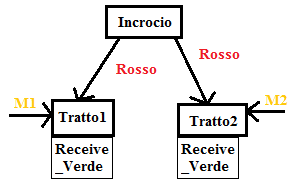
\includegraphics{./img/Semaforo1.png}
\caption{Semaforo 1}
\label{fig:Semaforo 1}
\end{center}
\end{figure}
Un attore inizia con il \lq receive\rq{} relativo al semaforo verde. Questo legge un mezzo ricevuto e lo rimanda al tratto o alla strada di destinazione. Supponiamo ora che l\textquoteright{}attore stia ricevendo dei mezzi ed un messaggio \lq Semaforo rosso\rq{} . All\textquoteright{}arrivo di un messaggio \lq Semaforo rosso\rq{} , questo verr\`{a} letto prima dei vari mezzi in arrivo.
\begin{figure}[H]
\begin{center}
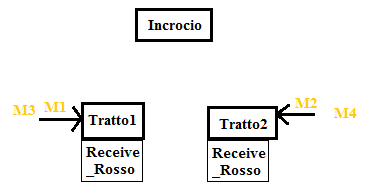
\includegraphics{./img/Semaforo2.png}
\caption{Semaforo 2}
\label{fig:Semaforo 2}
\end{center}
\end{figure}
Quel messaggio far\`{a} cambiare mailbox all\textquoteright{}attore. Gli altri messaggi non ancora gestiti verranno quindi letti con la nuova mailbox. 
\begin{figure}[H]
\begin{center}
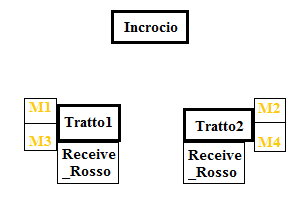
\includegraphics{./img/Semaforo3.png}
\caption{Semaforo 3}
\label{fig:Semaforo 3}
\end{center}
\end{figure}
Tale mailbox ora ha il compito di salvare tutti i mezzi in arrivo, simulando quindi la coda che si forma quando c\textquoteright{}\`{e} un semaforo rosso.
\begin{figure}[H]
\begin{center}
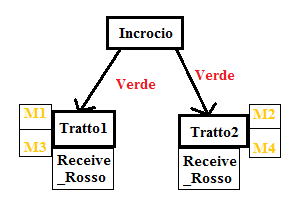
\includegraphics{./img/Semaforo4.png}
\caption{Semaforo 4}
\label{fig:Semaforo 4}
\end{center}
\end{figure}
Supponendo ora che arrivi un messaggio \lq Semaforo verde\rq{} , lo stato dell\textquoteright{}attore cambier\`{a} nuovamente.
\begin{figure}[H]
\begin{center}
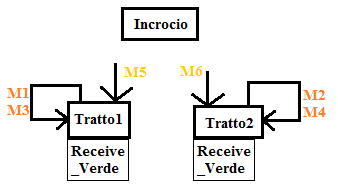
\includegraphics{./img/Semaforo5.png}
\caption{Semaforo 5}
\label{fig:Semaforo 5}
\end{center}
\end{figure}
Siccome i messaggi gi\`{a} letti non possono pi\`{u} essere letti dalla prima mailbox, dovranno essere rimandati. Per fare funzionare il tutto, i mezzi gi\`{a} accodati verranno rispediti con una priorit\`{a} un po\textquoteright{} pi\`{u} alta. Dunque prima di terminare la gestione del messaggio relativo al semaforo, si dovr\`{a} inviare all\textquoteright{}attore stesso TUTTI i mezzi accodati. Nell\textquoteright{}esempio dunque, \lq Tratto1\rq{} gestir\`{a} prima \lq M1\rq{} ed \lq M3\rq{} in quanto hanno priorit\`{a} media (\lq M1\rq{} verr\`{a} gestito per primo in quanto una \lq BoundedStablePriorityMailbox\rq{} garantisce il corretto ordinamento per i messaggi con la stessa priorit\`{a} ricevuti dallo stesso mittente) per poi gestire \lq M5\rq{} . Nel caso arrivasse un nuovo messaggio \lq Semaforo rosso\rq{} , la situazione verr\`{a} gestita come gi\`{a} spiegato all\textquoteright{}inizio. Tutti i mezzi non ancora gestiti verranno quindi letti con la seconda mailbox e verranno accodati.
\par La gestione dei semafori inoltre risulta molto semplice. Basta solo impostare un timer per poter inviare a se stesso un messaggio per fare scattare i semafori. Tale messaggio per\`{o} dovr\`{a} essere letto subito (e dovr\`{a} quindi avere una maggiore priorit\`{a} rispetto a mezzi e pedoni), quindi ci sar\`{a} bisogno di una \lq PriorityMailbox\rq{} anche per l\textquoteright{}incrocio.
\par La progettazione \`{e} stata fatta in modo tale da rendere il sistema pi\`{u} scalabile possibile. Esso infatti funziona con una quantit\`{a} qualsiasi di strade, di fermate, di mezzi e di persone. Questo perch\'{e} ogni componente dovr\`{a} comunicare solamente con un\textquoteright{}altra entit\`{a}.
\begin{figure}[H]
\begin{center}
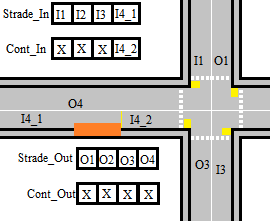
\includegraphics{./img/Strade2.png}
\caption{Strade 2}
\label{fig:Strade 2}
\end{center}
\end{figure}
Ogni strada infatti dovr\`{a} solo guardare se nella STESSA posizione della lista Cont\_In o Cont\_Out c\textquoteright{}\`{e} o meno un riferimento. Ovviamente ci dovr\`{a} essere un controllo per evitare che la strada \lq I4\_2\rq{} continui a mandare un messaggio sempre a se stessa. Dato che si era deciso di permettere al massimo una divisione per una strada, baster\`{a} controllare, ad esempio, se l\textquoteright{}identificativo della strada contiene \lq \_2\rq{}  alla fine. In tal caso comunicher\`{a} con quella strada, altrimenti comunicher\`{a} con l\textquoteright{}incrocio o con la zona vicina a seconda se la strada \`{e} \lq entrante\rq{} oppure \lq uscente\rq{} . Baster\`{a} quindi, durante la creazione delle strade, impostare correttamente i destinatari dei messaggi. Ogni zona potr\`{a} quindi avere un numero arbitrario di strade e ci potr\`{a} essere fino ad una fermata per ogni strada.
\par Come gi\`{a} detto inoltre, non \`{e} necessario l\textquoteright{}utilizzo di liste per poter salvare mezzi e pedoni. Tali code saranno infatti gestite automaticamente dalle mailbox dei vari attori (che gestiscono in maniera automatica l\textquoteright{}ordinamento. Akka infatti garantisce la lettura ordinata dei messaggi ricevuti dallo stesso mittente). 
\par Tale progettazione inoltre non comporta accodamenti forzati. Nessuna componente del sistema infatti deve aspettare che altre componenti finiscano il loro lavoro per poter continuare il proprio (ad eccezione dell\textquoteright{}incrocio con la gestione delle precedenze). 


\subsubsection{Distribuzione}
- Sincronizzazioni iniziali \newline
- Caduta zone \newline


\lettrine[lines=1]{P}{}er la realizzazione del sistema si vuole utilizzare il Clustering di Akka. Ogni cluster rappresenta un insieme di nodi (la cui posizione non \`{e} necessariamente nota al programmatore). L\textquoteright{}Akka Clustering \`{e} stato preferito rispetto all\textquoteright{}Akka Remoting in quanto, con quest\textquoteright{}ultimo, ci sarebbe l\textquoteright{} obbligato a conoscere gli indirizzi IP di tutte le zone. Nonostante ogni zona venga assegnata ad un nodo diverso, tutte le zone fanno parte dello stesso Actor System. In questo modo, ogni zona pu\`{o} richiedere (tramite un semplice \lq contex.actorSelection(…)\rq{} ) e ricevere i riferimenti alle zone vicine. Tali riferimenti verranno quindi utilizzati dalle varie componenti per permettere l\textquoteright{}invio di mezzi e persone.
\par La normale comunicazione tra le varie zone, dato che avviene tramite messaggi, utilizza una semantica \lq at-most-once\rq{} . Questo non va bene in quanto non \`{e} garantito l\textquoteright{}arrivo e la conseguente lettura dei messaggi da parte delle altre zone. Prima di poter dunque eliminare definitivamente un mezzo da una zona, bisogna essere certi che quella vicina l\textquoteright{}abbia ricevuto correttamente. Una semplice soluzione sarebbe quella di utilizzare il trait \lq AtLeastOnceDelivery\rq{} , ma esso comporta la gestione automatica di ulteriori invii in seguito a dei fallimenti, non garantendo pi\`{u} quindi il corretto ordinamento dei messaggi. Si \`{e} optato quindi per l\textquoteright{}utilizzo dei Futures. Ogni corsia o marciapiede dovr\`{a} aspettare una risposta dalla zona di destinazione prima di poter inviare il mezzo successivo. In caso la risposta non venga ricevuta in tempo, si dovr\`{a} ritentare con un nuovo invio. Ovviamente ogni zona dovr\`{a} essere in grado di scartare eventuali duplicati tramite l\textquoteright{}uso delle liste \lq mezziRicevuti\rq{} e \lq personeRicevute\rq{} . 
\begin{figure}[H]
\begin{center}
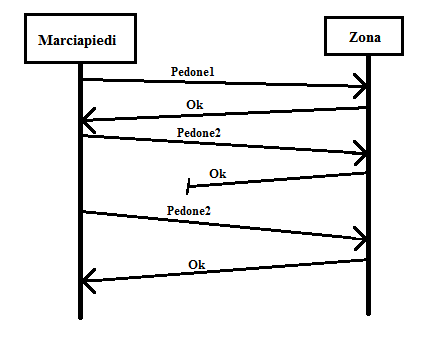
\includegraphics{./img/Protocollo.png}
\caption{Invio pedoni}
\label{fig:Invio pedoni}
\end{center}
\end{figure}
Questo pu\`{o} causare dei rallentamenti, ma consentir\`{a} al sistema di funzionare correttamente. L\textquoteright{}importante \`{e} non scegliere un tempo di attesa troppo breve (non voglio inviare troppi messaggi inutili), ma nemmeno troppo esteso (non voglio causare troppi rallentamenti solo per aspettare un messaggio).
\par La progettazione \`{e} stata fatta in modo tale da rendere il sistema pi\`{u} scalabile possibile. Il sistema infatti funziona con una quantit\`{a} qualsiasi di zone. Come gi\`{a} spiegato per la parte concorrente infatti, baster\`{a} passare i riferimenti corretti alle strade uscenti durante la fase di creazione per poter avere un numero arbitrario di zone.

\subsubsection{Lista e descrizione classi}

Aggiorno con VeicoloPiùpriorità, MezzoDeviato, ecc...



\begin{figure}[H]
\begin{center}
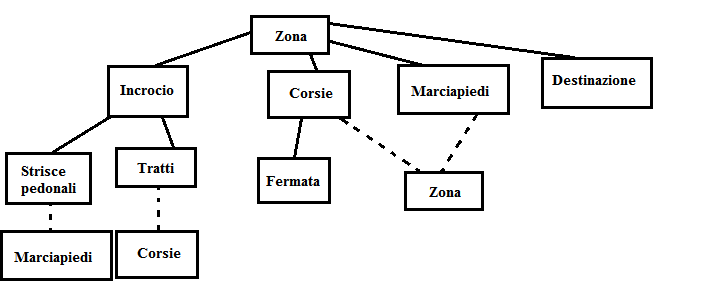
\includegraphics[ width=350px]{./img/Schema2.png}
\caption{Schema}
\label{fig:Schema}
\end{center}
\end{figure}
\lettrine[lines=1]{D}{}i seguito verranno elencate le classi da utilizzare nel progetto e le loro descrizioni. 
\begin{itemize}
\item {Zona:}
Classe che estende \lq Actor\rq{} e che rappresenta una zona. Riceve mezzi e persone e li passa all\textquoteright{}attore corretto. 
\item {Corsia:}
Classe che estende \lq Actor\rq{} e che rappresenta una corsia. Tale corsia pu\`{o} andare da una zona (o da un\textquoteright{}altra corsia) ad un incrocio o viceversa. Ogni corsia funziona grazie ad un gestore (uno per ogni corsia). Non appena tali gestori ricevono un mezzo, questi ne controllano il tipo e la destinazione ed inviano il mezzo dove necessario
\item {Fermata:}
Classe che estende \lq Actor\rq{} e che rappresenta la fermata per gli autobus. Alcune classi (come \lq Corsia\rq{} , \lq Marciapiede\rq{} e \lq Fermata\rq{} ) non hanno bisogno di liste di mezzi o di persone per funzionare correttamente. Tali classi infatti rappresentano degli attori con una propria mailbox. Tale attore ricever\`{a} molti messaggi, ma questi verranno accodati in automatico nella mailbox ed esaminati uno ad uno. Questo scelta \`{e} stata fatta in quanto Akka garantisce l\textquoteright{}ordinamento automatico di messaggi che arrivano dallo stesso mittente. In questo caso una corsia ricever\`{a} mezzi sempre dallo stesso mittente (o dalla sua zona). Nel secondo caso, ci saranno messaggi provenienti dalla zona alternati ad altri. Questa scelta modella il fatto di avere auto che si immettono in una certa strada. Stesso discorso vale per la fermata, che ricever\`{a} mezzi sempre dalla stessa corsia.
\item {Marciapiede:}
Classe che estende \lq Actor\rq{} e che rappresenta un marciapiede. Tale marciapiede pu\`{o} andare da una zona (o da un\textquoteright{}altra marciapiede) ad un incrocio o viceversa. I marciapiedi funzionano allo stesso modo delle corsie, con la sola differenza che non \`{e} previsto la divisione dei marciapiedi.
\item {Destinazione:}
Classe che estende \lq Actor\rq{} e che rappresenta l\textquoteright{}arrivo a destinazione di un mezzo o di un pedone. Per poter simulare l\textquoteright{}arrivo a destinazione, si \`{e} pensato di utilizzare una classe Destinazione. Essa assomiglia ad una specie di deposito dove i mezzi ed i pedoni arrivati a destinazione verranno inviati. Dopo un po\textquoteright{} di tempo questi verranno inviati nuovamente alla zona, che li instrader\`{a} correttamente per poter tornare indietro.
\item {Incrocio:}
Classe che estende \lq Actor\rq{} e che rappresenta un incrocio. Funziona allo stesso modo delle zone, ovvero riceve mezzi e persone e li passa all\textquoteright{}attore corretto.
\item {Tratto:}
Classe che estende \lq Actor\rq{} e che rappresenta i tratti dell\textquoteright{}incrocio. Il secondo pezzo corrisponde ai 4 tratti interni all\textquoteright{}incrocio. Essi funzionano in maniera simile alle corsie e alle strisce pedonali, con l\textquoteright{}unica differenza che comunicano tutte tra di loro. Non appena ricevono un mezzo, lo manderanno ad un altro tratto. 
Inoltre \lq Tratto\rq{} e \lq StrisciaPedonale\rq{} avranno due stati (due metodi \lq receive\rq{} ) per poter gestire correttamente gli invii, uno da usare quando il semaforo \`{e} rosso e l\textquoteright{}altro da usare quando il semaforo \`{e} verde. Il primo ricever\`{a} i mezzi e li salva nella coda. Appena ricever\`{a} un messaggio (semaforo verde), cambier\`{a} stato. Il secondo dunque invier\`{a} i mezzi in coda ed eventuali nuovi mezzi ricevuti finché non ricever\`{a} un certo messaggio (semaforo rosso). In questo caso si ritorner\`{a} al primo metodo \lq receive\rq{} .
Per gestire correttamente i semafori e quindi fermare subito il trasferimento dei mezzi, l\textquoteright{}attore necessita di una mailbox particolare. Sar\`{a} infatti necessario l\textquoteright{}utilizzo di una \lq BoundedStablePriorityMailbox\rq{} in quanto essa gestisce messaggi con priorit\`{a}, garantendo al tempo stesso l\textquoteright{}ordinamento corretto di messaggi con la stessa priorit\`{a}. 
L\textquoteright{}idea alla base dei semafori \`{e} la seguente: 
Messaggi \lq semaforo rosso\rq{} e \lq semaforo verde\rq{} avranno priorit\`{a} massima
Messaggi per l\textquoteright{}invio dei mezzi avranno priorit\`{a} minima
All\textquoteright{}arrivo di un messaggio \lq semaforo verde\rq{} , l\textquoteright{}attore invier\`{a} verso se stesso i mezzi accodati (in modo da essere letti con il secondo \lq receive\rq{} ), questa volta per\`{o} con priorit\`{a} media. In questo modo i mezzi gi\`{a} accodati saranno guardati ed inviati prima rispetto agli ultimi arrivati, ma saranno comunque analizzati dopo eventuali messaggi relativi al semaforo
All\textquoteright{}arrivo di un messaggio \lq semaforo rosso\rq{} , questo verr\`{a} letto subito, ed i mezzi che non sono ancora stati trasferiti saranno nuovamente accodati (prima quelli con priorit\`{a} media, non cambiando quindi l\textquoteright{}ordine della coda) subito dopo la fine dell\textquoteright{}invio in corso
\item {StrisciaPedonale:}
Classe che estende \lq Actor\rq{} e che rappresenta le strisce pedonali. Queste funzionano in maniera simile ai tratti ed alle corsie. Ricevono un pedone e lo mandano alle strisce pedonali successive (se questo deve effettivamente continuare). L\textquoteright{}unica diffrerenza rispetto alle corsie sta nel fatto che le strisce pedonali funzionano o meno in base ai semafori. L\textquoteright{}incrocio infatti avviser\`{a} le strisce pedonali quando dovranno cominciare a trasferire pedoni oppure quando dovranno smettere.
\lq Tratto\rq{} e \lq StrisciaPedonale\rq{} avranno due stati (due metodi \lq receive\rq{} ) per poter gestire correttamente gli invii, uno da usare quando il semaforo \`{e} rosso e l\textquoteright{}altro da usare quando il semaforo \`{e} verde. Il primo ricever\`{a} i pedoni e li salva nella coda. Appena ricever\`{a} un messaggio (semaforo verde), cambier\`{a} metodo \lq receive\rq{} . Il secondo dunque invier\`{a} i pedoni in coda ed eventuali nuovi mezzi ricevuti finché non ricever\`{a} un certo messaggio (semaforo rosso). In questo caso si ritorner\`{a} al primo metodo \lq receive\rq{} . Invio e accodamento funzioneranno esattamente come quelli nella classe \lq Tratto\rq{} .
\item {Persona:}
Trait che rappresenta una persona generica.
\item {PersonaDeviata:}
Classe che estende il trait \lq Persona\rq{} e che rappresenta per una persona che deve compiere una deviazione a causa di una zona non raggiungibile. 
\item {PersonaPi\`{u}Priorit\`{a}:}
Classe che contiene una persona. Questa classe viene utilizzata nelle strisce pedonali per poter gestire correttamente l'ordine dei pedoni e rappresenta semplicemente un pedone con una priorit\`{a} maggiore (come \`{e} gi\`{a} stato spiegato nella sezione \ref{Concorrenza}).
\item {Pedone:}
Classe che estende il trait \lq Persona\rq{} e che rappresenta per l\textquoteright{}appunto un pedone. 
\item {Mezzo:}
Trait che rappresenta un mezzo generico.
\item {MezzoPi\`{u}Priorit\`{a}:}
Classe che contiene un mezzo. Questa classe viene utilizzata nei tratti per poter gestire correttamente l'ordine dei mezzi e rappresenta semplicemente un mezzo con una priorit\`{a} maggiore (come \`{e} gi\`{a} stato spiegato nella sezione \ref{Concorrenza}).
\item {MezzoDeviato:}
Classe che estende il trait \lq Mezzo\rq{} e che rappresenta per un mezzo che deve compiere una deviazione a causa di una zona non raggiungibile. 
\item {Auto:}
Classe che estende il trait \lq Mezzo\rq{} e che rappresenta per l\textquoteright{}appunto una automobile. 
\item {Autobus:}
Classe che estende il trait \lq Mezzo\rq{} e che rappresenta per l\textquoteright{}appunto un autobus. 
\item {Classi container:}
Sono classi utilizzate per poter distinguere correttamente dello stesso tipo che devono essere utilizzati in maniera diversa. 








\color{red}\item {MapActor:} classe che facilita l'invio dei messaggi ad altre zone. Dato che ogni zona non sa in che cluster sono le altre, 









\end{itemize}
\subsubsection{Correttezza ordinamento messaggi}
- Scrivo che ogni messaggio arriva prima di altri (aggiorno con la sincronizzazione iniziale)


Di seguito verr \`{a} analizzata la correttezza dell\textquoteright{}ordinamento dei messaggi ricevuti dai vari attori.  \`{e} importante infatti che i messaggi arrivino nel corretto ordine e che l\textquoteright{}ordine dei mezzi e dei pedoni non cambi all\textquoteright{}improvviso.
\begin{itemize}
\item {corsiaOut -\textgreater{} zona:} non importa l\textquoteright{}ordine in cui una zona riceve i mezzi (e l\textquoteright{}ordine da una certa corsiaOut  \`{e} garantito)
\item {corsiaIn -\textgreater{} Incrocio:} non importa l\textquoteright{}ordine in cui l\textquoteright{}incrocio riceve i mezzi (e l\textquoteright{}ordine da una certa corsiaIn  \`{e} garantito)
\item {strada -\textgreater{} continuazione strada:} continuazione strada riceve mezzi solo da una corsia (sempre la stessa) e da una zona. Messaggi provenienti dalla zona possono mescolarsi a quelli provenienti dalla corsia (le macchine possono immettersi in strada da propriet \`{a} private ad esempio)
\item {tratto -\textgreater{} corsiaOut:} corsiaOut riceve mezzi solo da un tratto (sempre lo stesso) e da una zona. Messaggi provenienti dalla zona possono mescolarsi a quelli provenienti dal tratto (le macchine possono immettersi in strada da propriet \`{a} private ad esempio)
\item {tratto -\textgreater{} se stesso:} succede quando un semaforo diventa verde. Il tratto deve inviare prima i mezzi gi \`{a} in coda e non gli ultimi arrivati. Per fare ci \`{o} viene usata un\textquoteright{}apposita mailbox che gestisce le priorit \`{a} e al tempo stesso garantisce l\textquoteright{}ordine per i messaggi con la stessa priorit \`{a}. In questo modo, appena il semaforo diventa verde, il tratto si invier \`{a} i mezzi in coda con una priorit \`{a} un po\textquoteright{} pi \`{e} alta, cos \`{i} da poter spedire i primi mezzi in coda e non gli ultimi arrivati 
\item {corsia -\textgreater{} destinazione:} non importa l\textquoteright{}ordine in cui destinazione riceve i mezzi
\item {destinazione -\textgreater{} zona:} non importa l\textquoteright{}ordine in cui la zona riceve i mezzi
\item {marciapiedeOut -\textgreater{} zona:} non importa l\textquoteright{}ordine in cui una zona riceve i pedoni (e l\textquoteright{}ordine da un certo marciapiedeOut  \`{e} garantito)
\item {marciapiedeIn -\textgreater{} Incrocio:} non importa l\textquoteright{}ordine in cui l\textquoteright{}incrocio riceve i pedoni (e l\textquoteright{}ordine da un certo marciapiedeIn  \`{e} garantito)
\item {striscie pedonali -\textgreater{} striscie pedonali:} le striscie pedonali ricevono pedoni solo dalle strisce pedonali precedenti (sempre le stesse) e da un incrocio. Messaggi provenienti dall\textquoteright{}incrocio possono mescolarsi a quelli provenienti dalle strisce pedonali senza problemi
\item {striscie pedonali -\textgreater{} marciapiedeOut:} marciapiedeOut ricevono pedoni solo dalle strisce pedonali (sempre le stesse) e da una zona. Messaggi provenienti dalla zona possono mescolarsi a quelli provenienti dalle strisce pedonali senza problemi
\item {striscie pedonali -\textgreater{} se stesse:} succede quando un semaforo diventa verde. Il tratto deve inviare prima i pedoni gi \`{a} in coda e non gli ultimi arrivati. Per fare ci \`{o} viene usata un\textquoteright{}apposita mailbox che gestisce le priorit \`{a} e al tempo stesso garantisce l\textquoteright{}ordine per i messaggi con la stessa priorit \`{a}. In questo modo, appena il semaforo diventa verde, il tratto si invier \`{a} i pedoni in coda con una priorit \`{a} un po\textquoteright{} pi \`{e} alta, cos \`{i} da poter spedire i primi pedoni in coda e non gli ultimi arrivati 
\item {marciapiede -\textgreater{} destinazione:} non importa l\textquoteright{}ordine in cui destinazione riceve i pedoni
\item {destinazione -\textgreater{} zona:} non importa l\textquoteright{}ordine in cui la zona riceve i pedoni
\end{itemize}
\subsection{Funzionalit\`{a} non implementate}
- Motivazioni \newline
- Salvataggio di stato ogni tanto (quando una zona torna su, dovrebbe avere un metodo di recupero dei mezzi che aveva) \newline
- Grafica (creazione, ogni corsia, marciapiede, tratto e striscia pedonale ha un riferimento ad una label che modificherebbe man mano) \newline
\subsection{Screenshots}
- Fermata autobus con pedoni che salgono e scendono \newline
- Code ai semafori \newline
- Caduta zone e deviazioni

\newpage

\pagestyle{fancy}

\lhead{
	\color{black}
	\bfseries \textsf{\normalsize Bibliografia\\} 
}
\chead{}
\rhead{
	\color{black}
	\bfseries \textsf{\normalsize v.\Versione\\} 
}
\section{Bibliografia}
\begin{itemize}
\item {[1]} Scala: \textit{http://www.scala-lang.org/documentation/}
\item {[2]} Akka: \textit{http://doc.akka.io/docs/akka/snapshot/scala.html}
\item {[3]} SBT: \textit{http://www.scala-sbt.org/}
\item {[4]} Sistemi Concorrenti e Distribuiti: \textit{http://www.math.unipd.it/$\sim$tullio/SCD/2014/}
\item {[5]} Routing: \textit{http://en.wikipedia.org/wiki/List\_of\_ad\_hoc\_routing\_protocols}
\end{itemize}
\begin{midpage}
\begin{center}
\null
\end{center}
\end{midpage}
\end{document}
